\documentclass[11pt]{article}
\usepackage{latexsym}
\usepackage{amsmath}
\usepackage{amssymb}
\usepackage{amsthm}
\usepackage{epsfig}
\usepackage[tight]{subfigure}

\usepackage{amsmath}

\DeclareMathOperator*{\minimize}{min}
\DeclareMathOperator*{\maximize}{max}

\usepackage{algorithm}
 %on linux you may need to run sudo apt-get install texlive-full to install algorithm.sys
\usepackage{algorithmic}

\usepackage{verbatim}

\newcommand{\handout}[5]{
  \noindent
  \begin{center}
  \framebox{
    \vbox{
      \hbox to 5.78in { {#1} \hfill #2 }
      \vspace{4mm}
      \hbox to 5.78in { {\Large \hfill #5  \hfill} }
      \vspace{2mm}
      \hbox to 5.78in { {\em #3 \hfill #4} }
    }
  }
  \end{center}
  \vspace*{4mm}
}

\newcommand{\lecture}[5]{\handout{#1}{#2}{#3}{#4}{#5}}
\newcommand{\collision}[0]{\mathrm{collision}}
\newcommand{\nocollision}[0]{\overline{\collision}}

\newcommand*{\QED}{\hfill\ensuremath{\square}}

\newtheorem{theorem}{Theorem}
\newtheorem{corollary}[theorem]{Corollary}
\newtheorem{lemma}[theorem]{Lemma}
\newtheorem{observation}[theorem]{Observation}
\newtheorem{proposition}[theorem]{Proposition}
\newtheorem{definition}[theorem]{Definition}
\newtheorem{claim}[theorem]{Claim}
\newtheorem{fact}[theorem]{Fact}
\newtheorem{assumption}[theorem]{Assumption}
\newtheorem{note}[theorem]{Note}

% 1-inch margins, from fullpage.sty by H.Partl, Version 2, Dec. 15, 1988.
\topmargin 0pt
\advance \topmargin by -\headheight
\advance \topmargin by -\headsep
\textheight 8.9in
\oddsidemargin 0pt
\evensidemargin \oddsidemargin
\marginparwidth 0.5in
\textwidth 6.5in

\parindent 0in
\parskip 1.5ex
%\renewcommand{\baselinestretch}{1.25}

\begin{document}

\lecture{Statistical Techniques in Robotics (16-831, S21)}{Lecture \#06
  (Wednesday, February 17)}{Lecturer: Kris Kitani}{Scribes: Roshni Kaushik and Cornelia Bauer}{Online Convex Optimization (Convexity, FTL)}

\section{Review}
\subsection{Online Learning}
Recall the goal of online learning (Figure \ref{fig:online_learning}) is to make a series of accurate predictions given a sequence of inputs. At each time step $t$, the learner takes in the input and any additional information (such as expert predictions). It then makes a prediction $\hat{y}$ that validates given a true label $y$. Based on the calculated loss between these two, it updates its parameters for the next time step. 
\begin{figure}[ht]
    \centering
    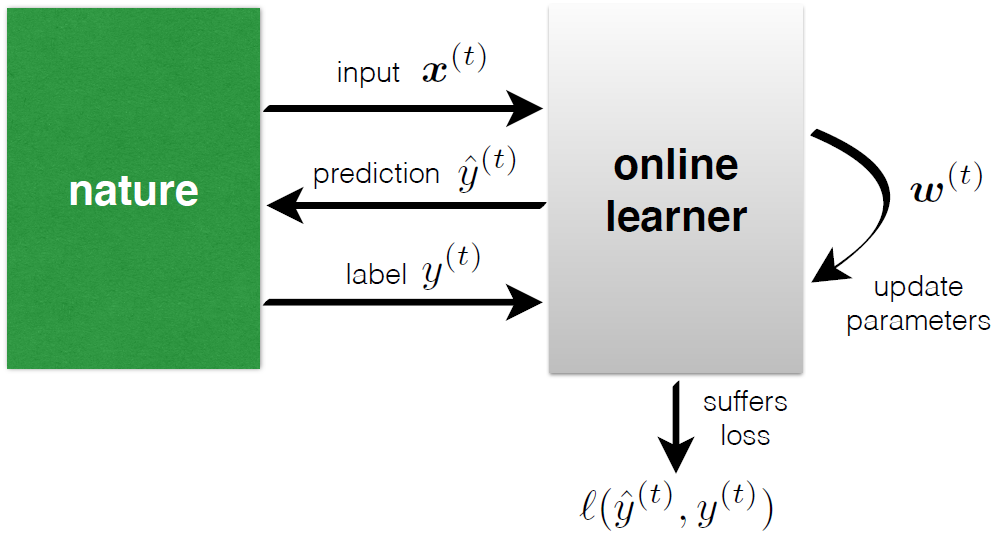
\includegraphics[width=0.7\textwidth]{online_learning}
    \caption{Online Learning (Lecture 6, Slide 16)}
    \label{fig:online_learning}
\end{figure}

Some topics we have discussed previously are the mistake and regret bounds of the online learning algorithms. Mistake bounds are the upper limit on the expected number of mistakes the algorithm can make. Regret bounds compare the expected loss of the learner with the best hypothesis $h \in \mathcal{H}$.

We have seen online learning algorithms in two different categories thus far. \emph{Greedy (Consistent)}, \emph{Halving}, \emph{Weighted Majority}, and \emph{Randomized Weighted Majority} Algorithms all fall under \textbf{Prediction with Expert Advice}. In this category, the learner is given a set of expert predictions at each time step. The second category is \textbf{Online Linear Classification}, and we have seen the \emph{Online Perceptron} and \emph{Winnow} Algorithm in this category.

\subsection{Convexity}

\definition{\normalfont A set $S$ is \textbf{convex} if for all $w, v \in S$, $\alpha w + (1 - \alpha) v \in S$ for all $\alpha \in [0, 1]$}
\normalfont
In two dimensions, this means that a set $S$ is convex if a line connecting any two points is contained within the set. Figure \ref{fig:convex_set} is an example of a convex set, and for any two points $X$ and $Y$, the line connecting it is always contained within the set.

\begin{figure}[ht]
    \centering
    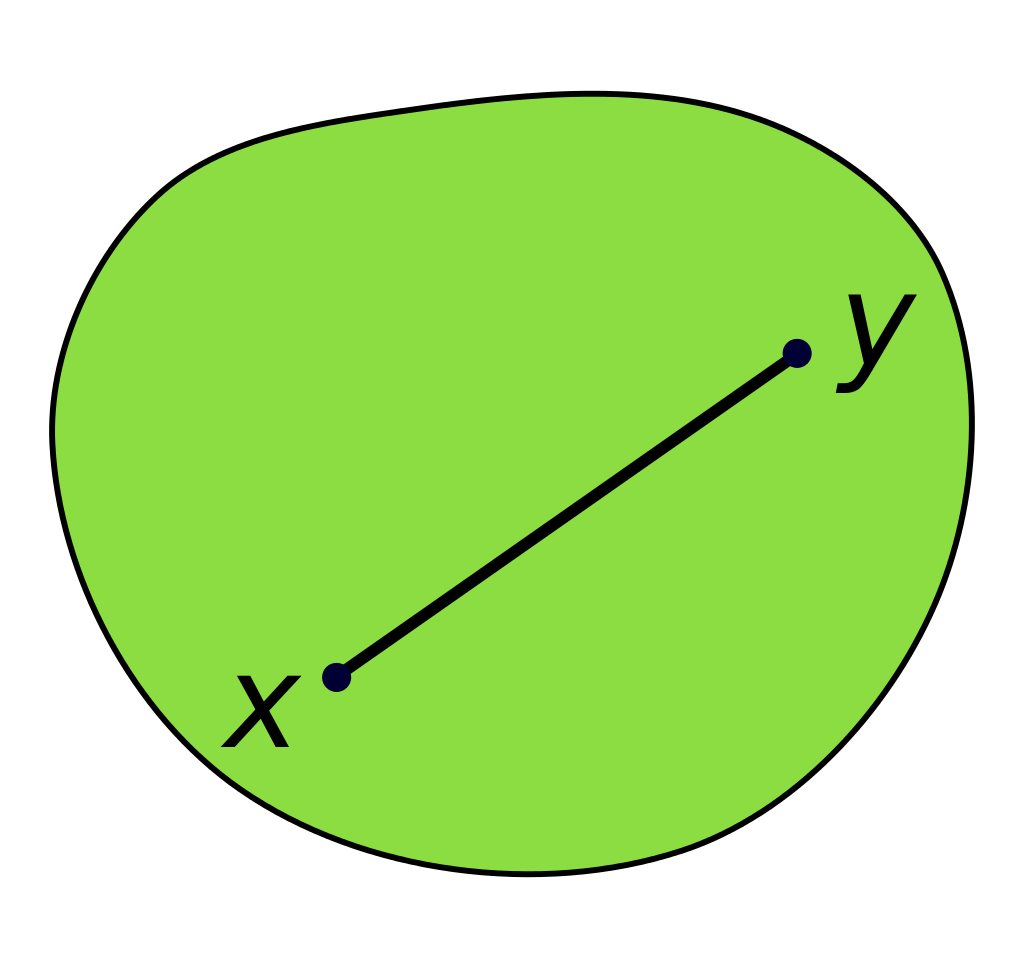
\includegraphics[width=0.5\textwidth]{convex_set}
    \caption{Convex Set (image from Wikipedia)}
    \label{fig:convex_set}
\end{figure}

\definition{\normalfont A function $f: S \in \mathbb{R}$ is \textbf{convex} if for all $w, v \in S$, $f(\alpha w + (1 - \alpha) v) \leq \alpha f(w) + (1 - \alpha) f(v)$ for all $\alpha \in [0, 1]$}

\normalfont
In two dimensions, this means that a convex function $f$ between any two points is upper-bounded by a line connecting the two points. Or that a line connecting two points on a convex function always lies above the function. Figure \ref{fig:convex_function} is an example of a convex function. The line connecting any two points $x_1$ and $x_2$ always lies above the function.

\begin{figure}[ht]
    \centering
    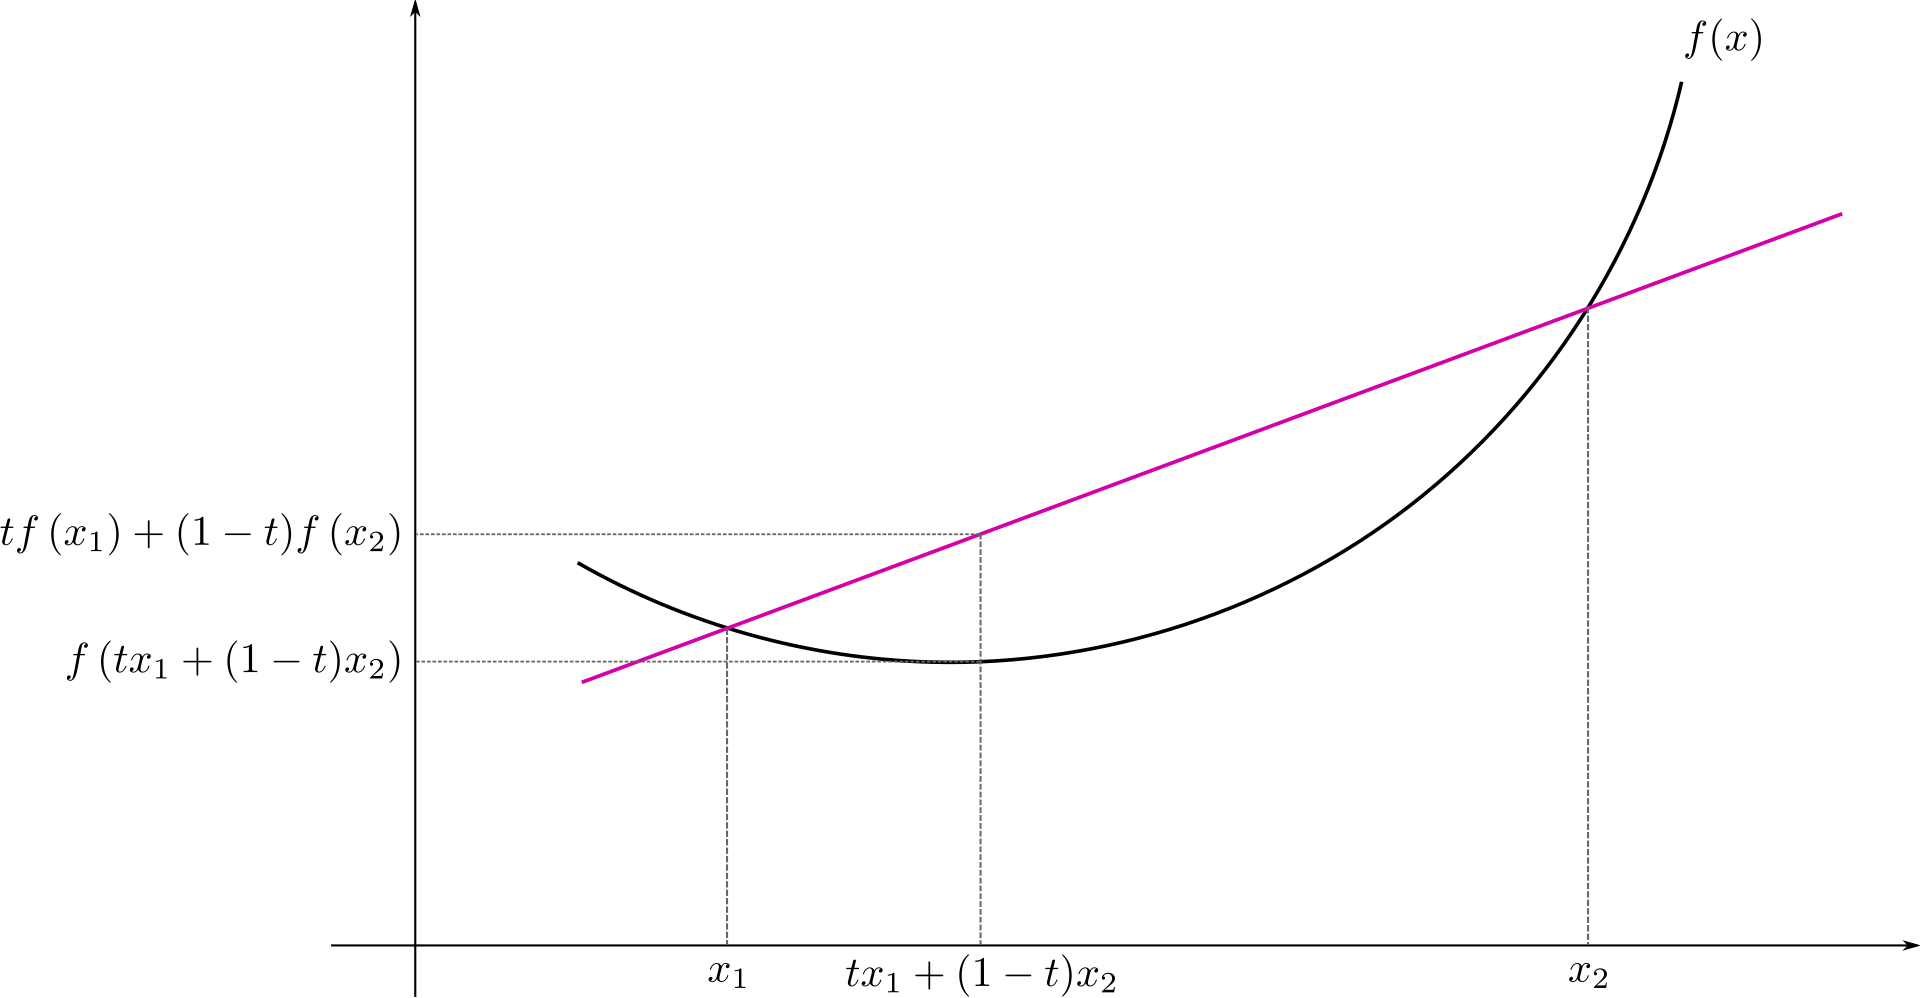
\includegraphics[width=0.4\textwidth]{convex_function}
    \caption{Convex Function (image from Wikipedia)}
    \label{fig:convex_function}
\end{figure}

\section{Summary}

\subsection{Optimization}
Optimization involves minimizing or maximizing a function by choosing valid inputs and computing the value of the function on those inputs. 

\definition{\normalfont A (constrained) optimization problem can be formulated as $\min f(x)$, with constraints $g(x) \leq 0;~h(x) = 0~x \in S$}

\normalfont
$g(x)$ is the inequality constraint, $h(x)$ is the equality constraint, and $S$ is the optimization domain. There are three solution methods for solving optimization problems, each with benefits and drawbacks.

\subsubsection*{Analytic Solution}
The analytic solution such as to $\nabla f(x) = 0$ can provide a global and fast solution to the optimization problem. However, it can be very difficult and sometimes impossible to compute.

\subsubsection*{Brute Force Search}
Brute force search involves testing all possible valid inputs, exhaustively, to find the optimal value. This approach has the benefit of providing a global solution, but is usually very slow for a large input space and is sometimes impossible depending on the formulation of the problem.

\subsubsection*{Numerical Methods}
Numerical methods, such as gradient descent, are a popular and sometimes fast way to solve optimization problems. However, these methods usually do not have guarantees for finding a global solution.

Numerical methods can be used to solve online convex optimization by:
\begin{enumerate}
    \item Receiving one data sample
    \item Observing the loss
    \item Update the parameters (weights)
\end{enumerate}

This process, using an online learner, is illustrated in Figure \ref{fig:online_convex_opt}.

\begin{figure}[ht]
    \centering
    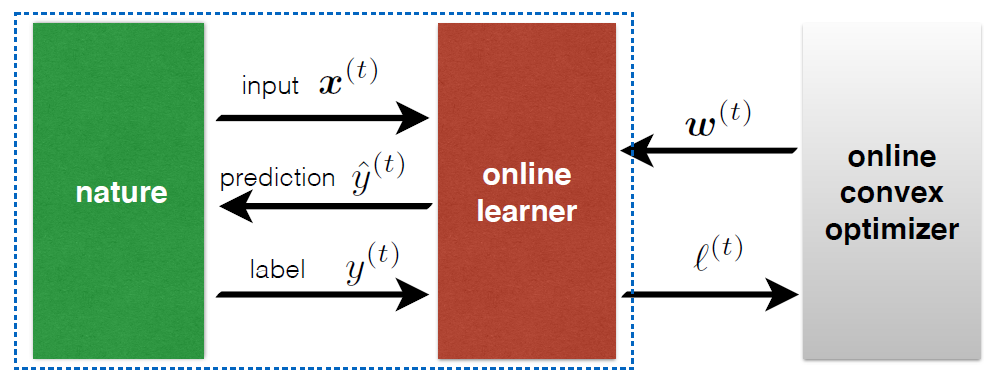
\includegraphics[width=0.7\textwidth]{online_convex_opt}
    \caption{Online Convex Optimization (Lecture 6, Slide 18)}
    \label{fig:online_convex_opt}
\end{figure}

\subsection{Lipschitz Continuity}
A function $f$ is called \textbf{L-Lipschitz} over a set $S$ with respect to a norm, if the following holds for all $\boldsymbol{u},\boldsymbol{w}\in S$

\begin{equation*}
    |f(\boldsymbol{u})-f(\boldsymbol{w})|\leq L||\boldsymbol{u}-\boldsymbol{w}||    
\end{equation*}
From Wikipedia \cite{wikiLipschitz}: Intuitively, Lipschitz continuity is a measure for how fast a function can change: There exists a real number such that, for every pair of points on the graph of this function, the absolute value of the slope of the line connecting them is not greater than this real number.

\begin{figure}[ht]
    \centering
    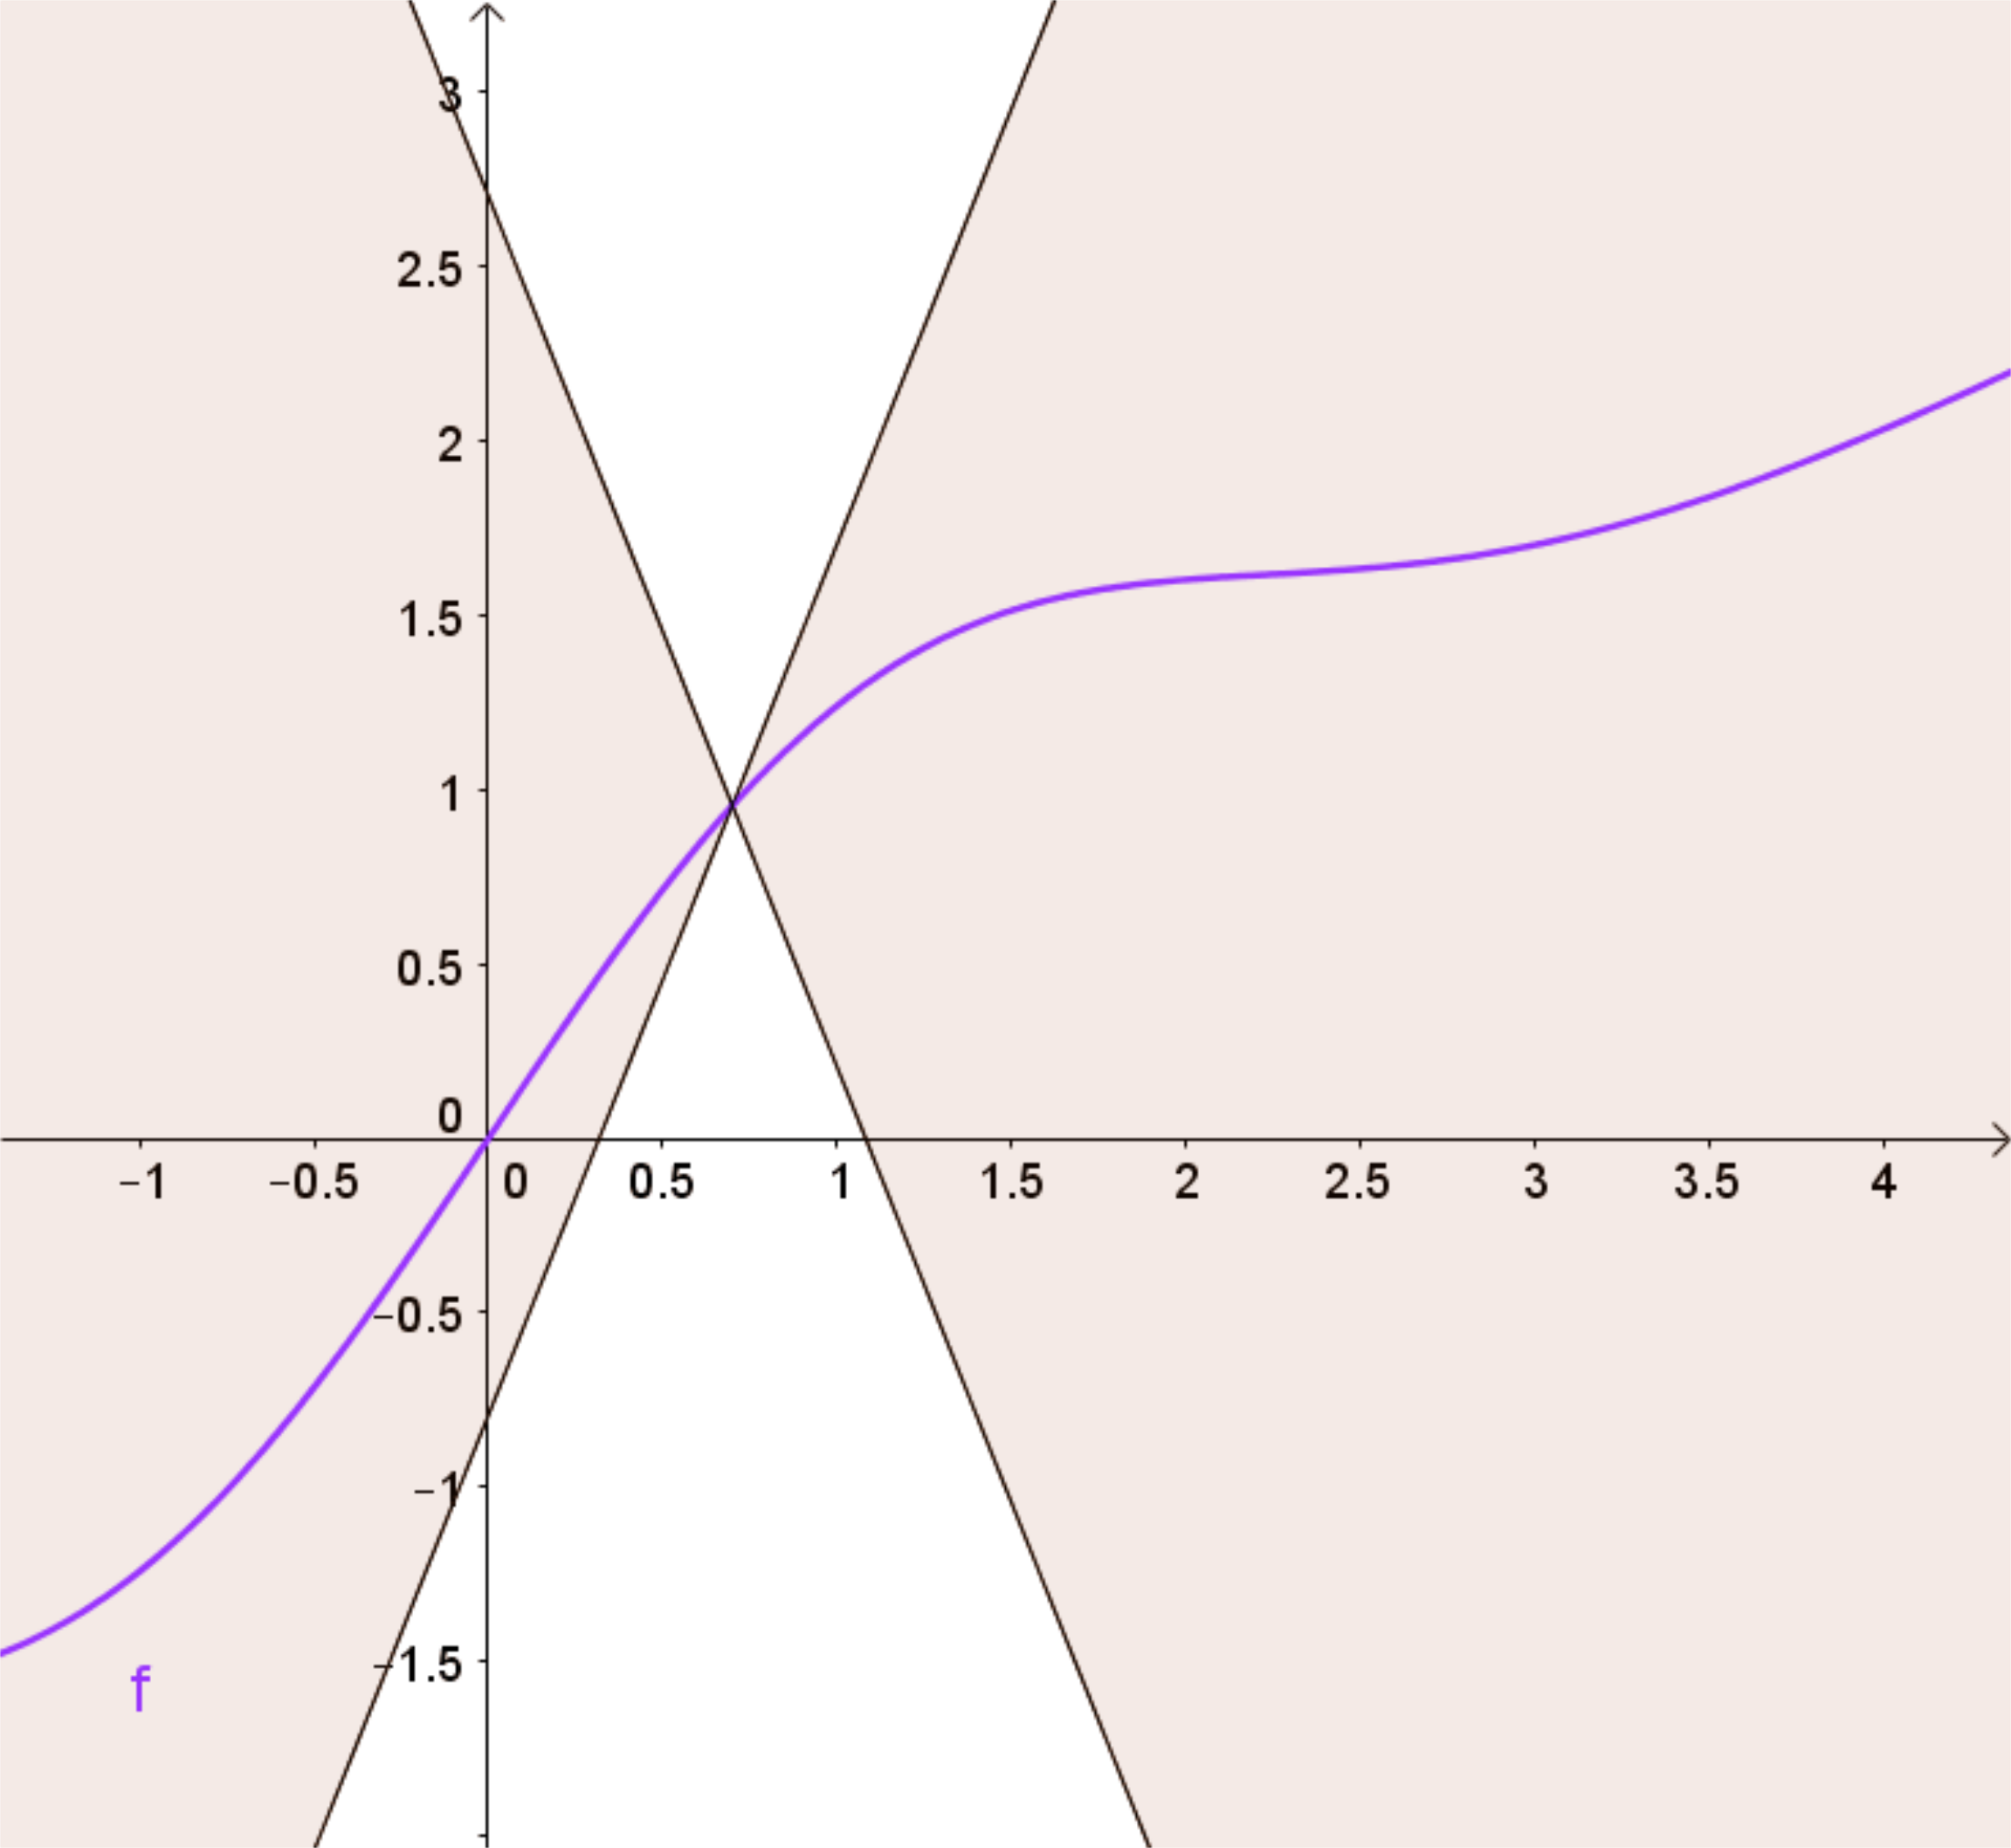
\includegraphics[width=0.3\textwidth]{Lipschitz.png}
    \caption{Lipschitz continuity visualization. From \cite{wikiLipschitz}.}
    \label{fig:lipschitz_cone}
\end{figure}

If a function is Lipschitz continuous, there exists a double cone (depicted in white in \ref{fig:lipschitz_cone}) whose origin can be moved along the graph such that the whole graph always stays outside of the double cone.

\subsection{Convexification}
There exist many problems and learning applications in which the loss function is not convex. We can however apply a few tricks to turn a non-convex loss function into a convex one. This process is called \textbf{convexification}, and we will summarize two methods in the following sections: Convexification by randomization and convexification by surrogate loss.

\subsubsection*{Convexification by randomization}
We will now consider the Weighted Majority Algorithm (WMA) (see Lecture 3 for more details). This algorithm predicts based on the majority vote 
\begin{equation*}
    \hat{y}=\text{sign} \langle \boldsymbol{x}^{(t)}, \boldsymbol{w}^{(t-1)}\rangle
\end{equation*}
and we receive a loss 
\begin{equation*}
    l^{(t)} = \mathbf{1}[\hat{y}^{(t)}\neq y^{(t)}]
\end{equation*}
This algorithm is a bounded-regret algorithm.
If we examine the parameter space, we realize that the parameter space is the set of positive real numbers, $\mathbb{R}^+$. This is a convex set.
However, the loss function is either zero or one, which is a non-convex function, as shown in Fig. \ref{fig:zero_one_loss}.
\begin{figure}[ht]
    \centering
    
\includegraphics[width=0.3\textwidth]{0_1_loss.png}
    \caption{Zero-One loss. Since the circled portion of the function is above the line segment, this problem is a non-convex function.}
    \label{fig:zero_one_loss}
\end{figure}
We will now show that we can use randomization to make this loss function convex. If we look at the prediction rule of the Randomized Weighted Majority Algorithm (RWMA)
\begin{equation*}
    h \sim \textsc{Multinomial}(\textbf{\textit{w}}^{(t)}/ \Phi^{(t)})
\end{equation*}
\begin{equation*}
    \hat{y}^{(t)} = h(\textbf{\textit{x}}^{(t)})
\end{equation*}
we predict based on a multinomial distribution over the relative expert weights $w^{(t)}$.
The parameter space here is the set of positive real numbers, $\mathbb{R}^+$. The loss function for RWMA is given by
\begin{equation*}
    l^{(t)}=E_p[\textbf{1}[y^{(t)}\neq \hat{y}_n^{(t)}]]=\sum_{p_n} p_n \textbf{1}[y^{(t)}\neq \hat{y}_n^{(t)}])
\end{equation*}
which can be visualized as shown in Fig. \ref{fig:linear_loss}.

\begin{figure}[ht]
    \centering
    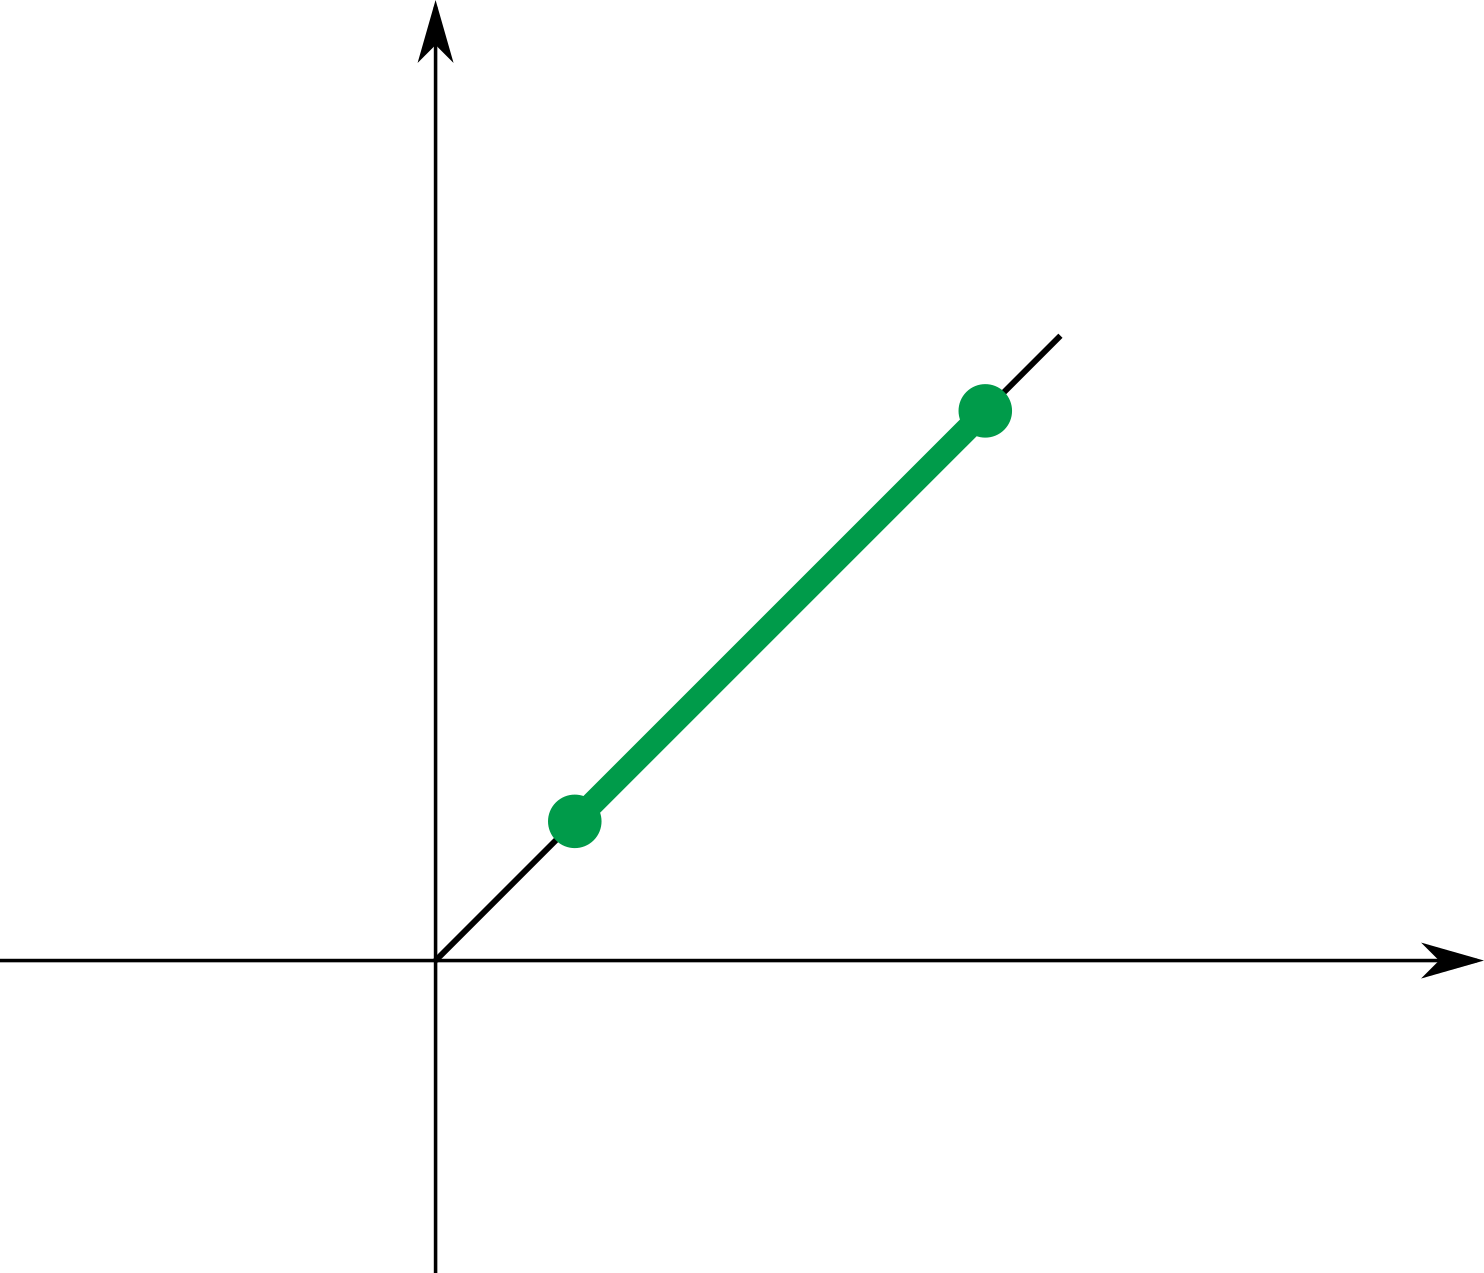
\includegraphics[width=0.3\textwidth]{linear_loss.png}
    \caption{Linear loss, a convex function.}
    \label{fig:linear_loss}
\end{figure}
We observe that this is a linear function, which is convex. We have therefore shown that by introducing randomization to the algorithm, we have transformed the loss function into a convex function. It should be noted that randomization also turned this algorithm from being bounded-regret into a no-regret algorithm.

\subsubsection*{Convexification by surrogate loss}
A further method to transform a non-convex problem into a convex problem is to replace the original non-convex loss function with a \textbf{surrogate} loss function. 

In order to apply this method, there are two requirements:

\begin{itemize}
    \item The surrogate loss upper bounds the original loss
    \item The surrogate loss is convex
\end{itemize}
If we now minimize the surrogate loss, we are minimizing an upper bound of the original loss.

For WMA, we can introduce the \textit{hinge} loss as a surrogate loss function. The hinge loss is given by the following equations.

\begin{align*}
    l^{(t)} &= \mathbf{1}[\hat{y}^{(t)}\neq y^{(t)}]\\
     &= \mathbf{1}[1-y^{(t)}\langle \boldsymbol{w}^{(t-1)},\boldsymbol{x}^{(t)}\rangle >1]\\
     &\leq     \text{max}\big[0,1-y^{(t)}\langle \boldsymbol{w}^{(t-1)},\boldsymbol{x}^{(t)}\rangle>1\big]\\
     \Tilde{l}^{(t)}&=\text{max}\big[0,1-y^{(t)}\langle \boldsymbol{w}^{(t-1)},\boldsymbol{x}^{(t)}\rangle>1\big]
\end{align*}
As shown in Fig. \ref{fig:hinge_loss}, the hinge loss $\Tilde{l}^{(t)}$ is a convex function.
We have therefore shown that the surrogate loss upper bounds the original loss, and turned this problem into a convex problem.

\begin{figure}[ht]
    \centering
    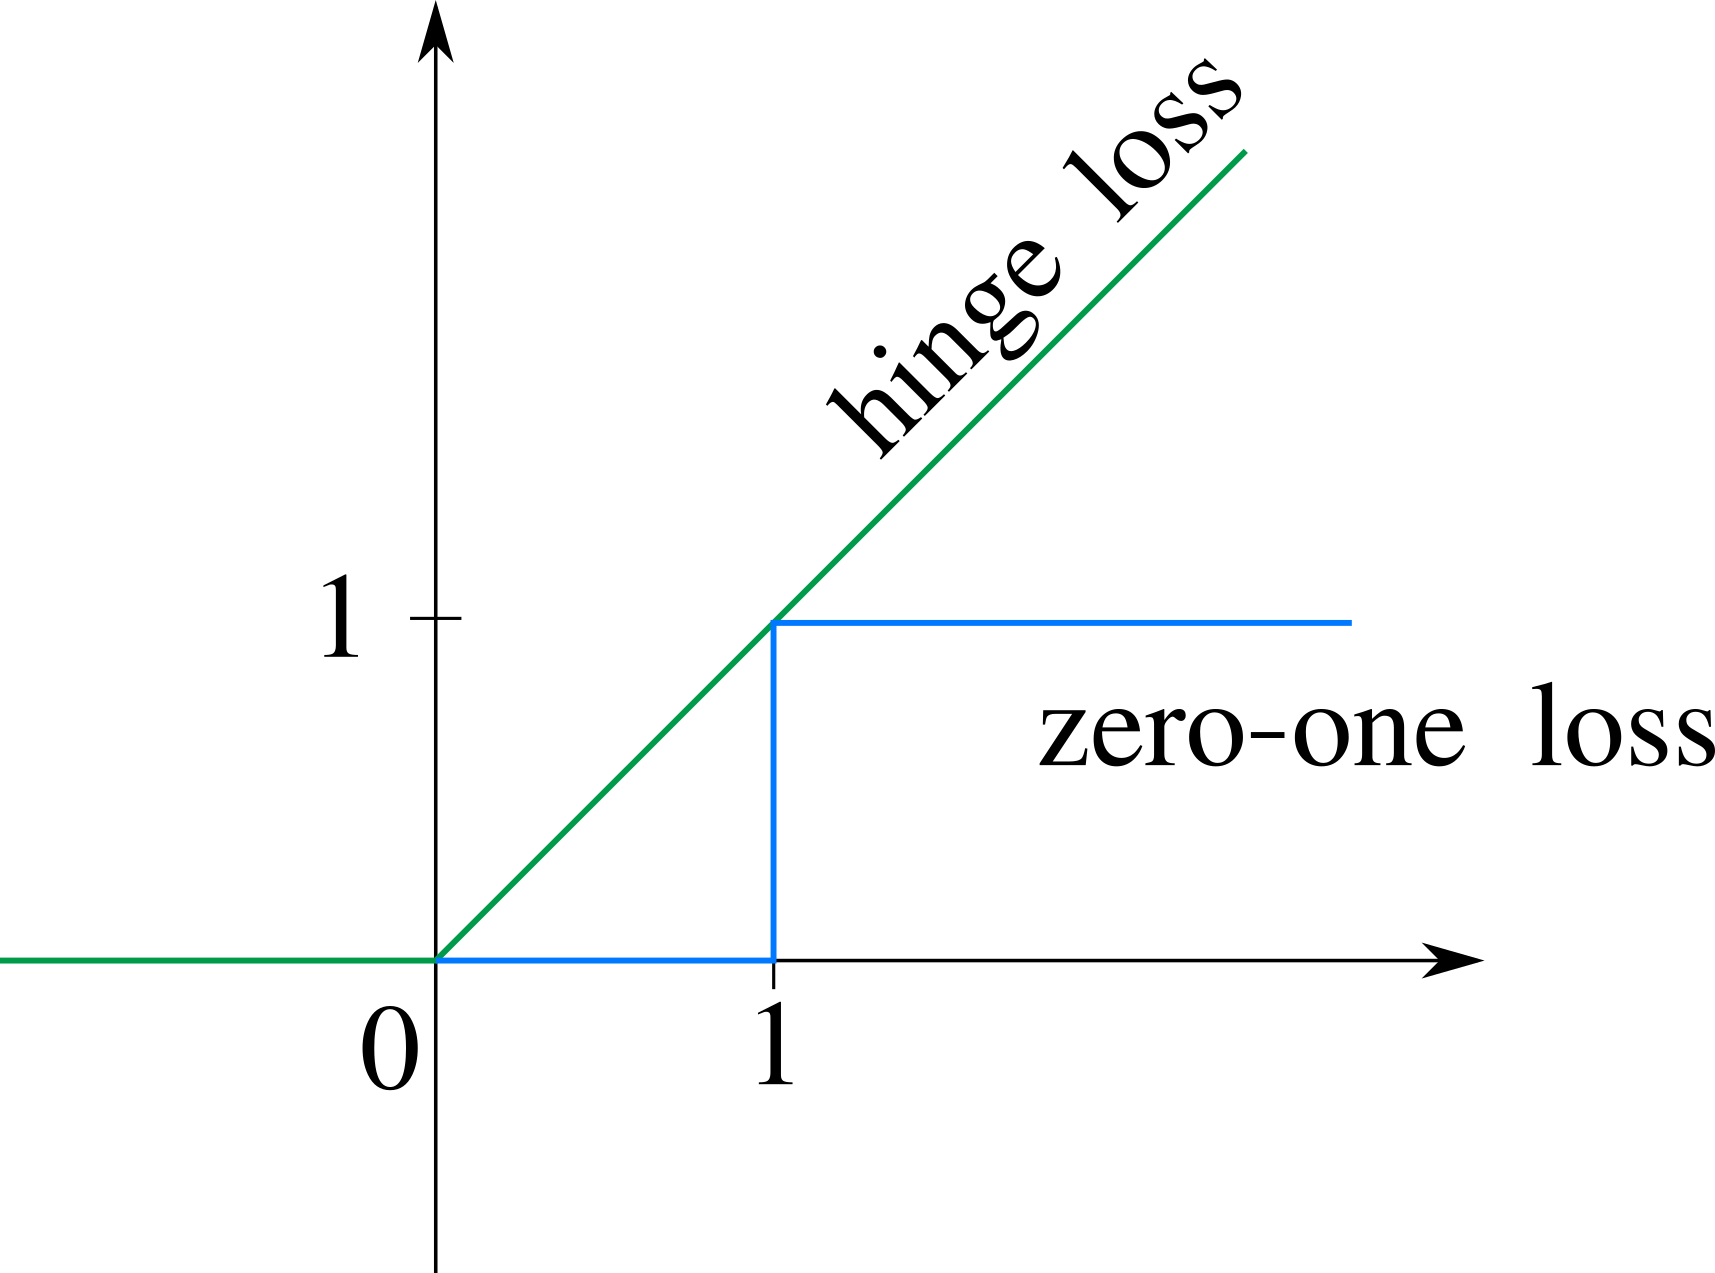
\includegraphics[width=0.3\textwidth]{hinge_loss.png}
    \caption{Hinge loss upper bounds zero-one loss and is a convex function.}
    \label{fig:hinge_loss}
\end{figure}


\subsection{Follow the Leader}
We will now discuss an algorithm for online convex optimization problems. Follow the leader (FTL), also termed \textit{Fictitious Play}, was first introduced by G. W. Brown in 1951 \cite{brown1951iterative,berger2007brown}.


\begin{algorithm}[H]
\caption{Follow the leader}
\label{algo:ftl}
\begin{algorithmic}[1]
\STATE $\textbf{function} \;\;\textsc{follow the leader} $
\STATE \qquad \textbf{for} {$t=1,2\;\cdots,\;T$} \textbf{do}
\vspace{5pt}
\STATE \qquad \qquad $\boldsymbol{w}^{(t)}=\text{arg min}_{\boldsymbol{w}\in W} \sum_{i=1}^{t-1} f^{(i)} (\boldsymbol{w})$
\vspace{5pt}
\STATE \qquad \qquad $\textsc{Receive}(f^{(T)}:W \rightarrow \mathbb{R})$
 \label{alg:wma_weight_update}
\end{algorithmic}
\end{algorithm}

The main idea of this algorithm is that the learner should go by the best choice seen so far. We can plug the weight update rule (line 3 in Algorithm \ref{algo:ftl}) into the online convex optimization as shown in Fig. \ref{fig:online_convex_opt}.

We will now derive the regret bound. For this purpose, we will introduce the concept of the \textbf{ one-step look ahead cheater}. 

The cumulative regret is given by

\begin{equation*}
    R(\boldsymbol{u})=\sum_t [f^{(t)}(\boldsymbol{w}^{(t)})-f^{(t)}(\boldsymbol{u})]
\end{equation*}
where $\boldsymbol{u}$ is any expert, $\boldsymbol{w}^{(t)}$ is the set of parameters at time $t$, $f^{(t)}$ the loss function returned to the online learner by nature. It is difficult to reason about $\boldsymbol{u}$ as there are infinite possibilities. We can however upper bound the regret by introducing a \textit{one step look ahead cheater} $\boldsymbol{w}^{(t+1)}$:

\begin{equation*}
    R(\boldsymbol{u})\leq \sum_t [f^{(t)}(\boldsymbol{w}^{(t)})-f^{(t)} (\boldsymbol{w}^{(t+1)})]
\end{equation*}

We will now prove that this inequality holds true. We start by subtracting $f^{(t)}(\boldsymbol{w}^{(t)})$ from both sides of the inequality, which leaves us with 


\begin{equation*}
    \sum_{t=1}^T f^{(t)} (\boldsymbol{w}^{(t+1)})\leq  \sum_{t=1}^T f^{(t)} (\boldsymbol{u})
\end{equation*}


This means that the loss of a series of one step cheaters is less than or equal to the loss of any other single parameter $\boldsymbol{u}$.

We can prove that this inequality holds true by Induction: 
We assume that the inequality holds for $T-1$
\begin{equation*}
    \sum_{t=1}^{T-1} f^{(t)} (\boldsymbol{w}^{(t+1)})\leq  \sum_{t=1}^{T-1} f^{(t)} (\boldsymbol{u}) \;\;\;\;\; \forall \boldsymbol{u}
\end{equation*}
If we add $f^{(T)}(\boldsymbol{w}^{(T+1)})$ to both sides, we obtain
\begin{equation*}
    \sum_{t=1}^{T} f^{(t)} (\boldsymbol{w}^{(t+1)})\leq f^{(T)}(\boldsymbol{w}^{(T+1)}) +  \sum_{t=1}^{T-1} f^{(t)} (\boldsymbol{u}) 
\end{equation*}
Note that the term can be consumed within the summation on the left hand side, but not on the right hand side, since the parameters are different. But since we assume that the inequality is true for all $\boldsymbol{u}$, we simply set it to $\boldsymbol{u}=\boldsymbol{w}^{(T+1)}$, and can write
\begin{align*}
       \sum_{t=1}^{T} f^{(t)} (\boldsymbol{w}^{(t+1)})&\leq f^{(T)}(\boldsymbol{w}^{(T+1)}) +  \sum_{t=1}^{T-1} f^{(t)} (\boldsymbol{w}^{(T+1)})\\
       &\leq \sum_{t=1}^{T} f^{(t)} (\boldsymbol{w}^{(T+1)})
\end{align*}
From this inequality we can derive that the loss of using the one-step look ahead cheater at each time step is upper bounded by the loss of using a single one-step look ahead cheater at the end of the sequence for all time steps. Given the definition of the minimizer, $\boldsymbol{w}^{(T+1)}= \underset{\boldsymbol{u}\in S}{\text{arg min}} \sum_{t=1}^T f^{(t)} (\boldsymbol{u})$
this means we can upper bound the right hand side of the inequality by all $\boldsymbol{u}$:

\begin{equation*}
           \sum_{t=1}^{T} f^{(t)} (\boldsymbol{w}^{(t+1)})
       \leq \sum_{t=1}^{T} f^{(t)} (\boldsymbol{u})
\end{equation*}

We can now plug this back into our original upper bound on the regret, and finally obtain
\begin{align*}
        R(\boldsymbol{u})&=\sum_t [f^{(t)}(\boldsymbol{w}^{(t)})-f^{(t)}(\boldsymbol{u})]\\
        &\leq \sum_t [f^{(t)}(\boldsymbol{w}^{(t)})-f^{(t)} (\boldsymbol{w}^{(t+1)})]
\end{align*}
which concludes our proof.
{
\bibliography{refs}
\bibliographystyle{abbrv}
}
\end{document} % Done!


